\begin{frame}{Traditional Numerical Methods in Geophysics}
\begin{columns}
\begin{column}{0.5\textwidth}
	\begin{figure}
	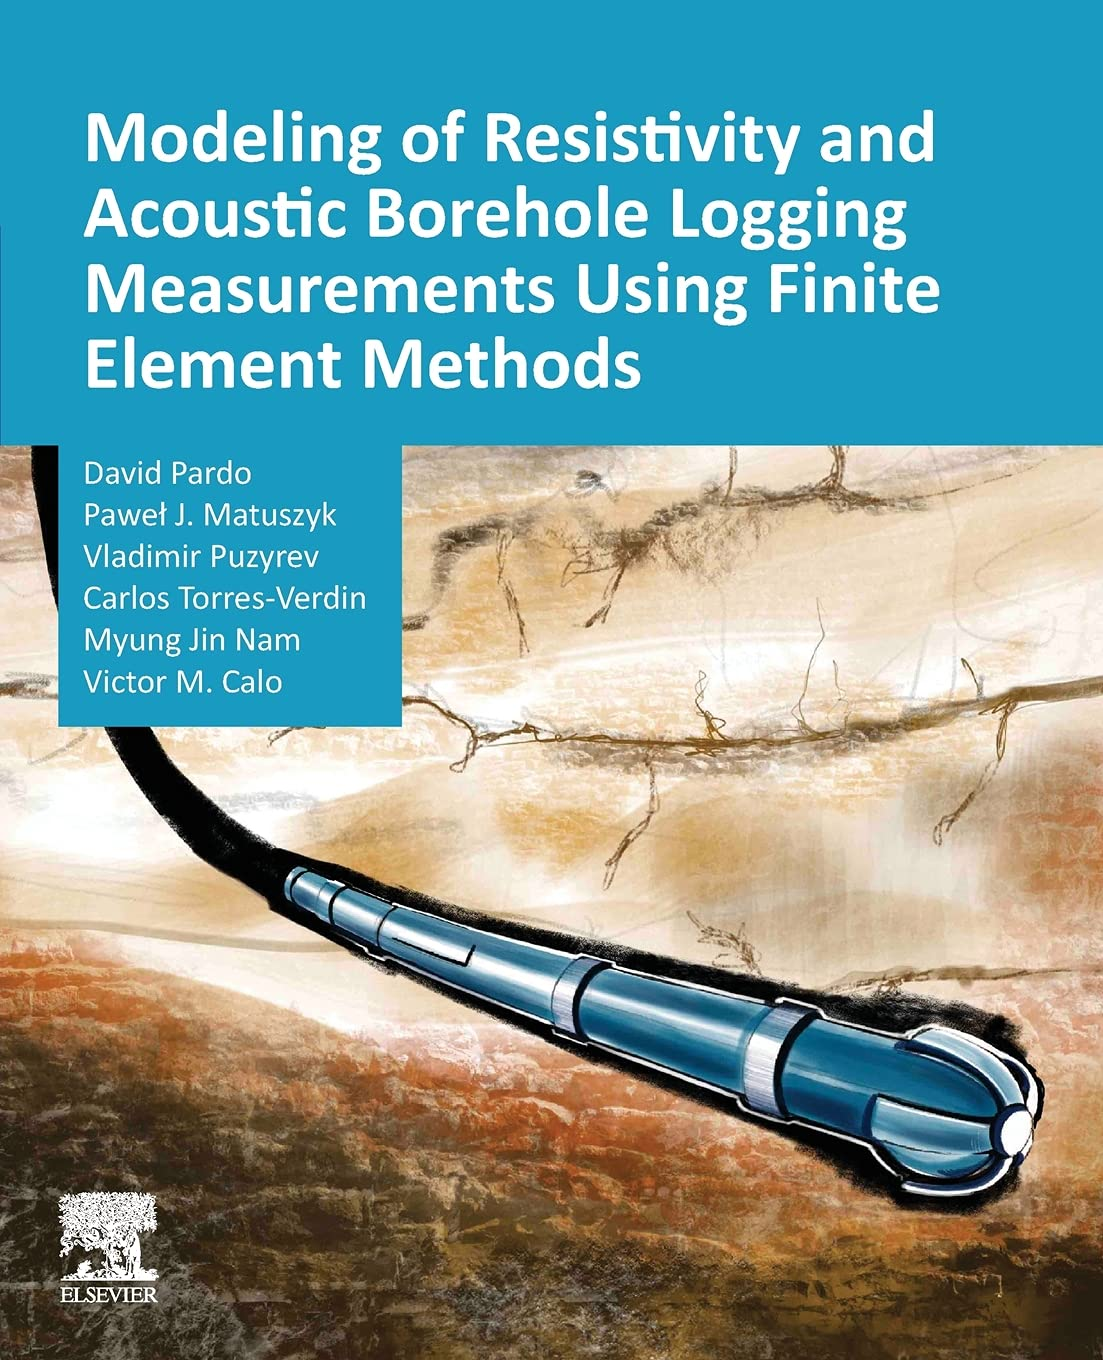
\includegraphics[scale=0.13]{frames/JonAnder/Figures/PardoBook.jpg}
	\end{figure}
	\hspace{0.9cm} {\small Published in 2021}
\end{column}
%
\begin{column}{0.5\textwidth}
\begin{itemize}
\item Finite Element method
\vspace{0.4cm}
\item Finite Difference method
\vspace{0.4cm}
\item Finite Volumes method
\vspace{0.4cm}
\item Integral methods
\vspace{0.4cm}
\item Semi-analytical methods
\end{itemize}
\end{column}
\end{columns}
\end{frame}

\begin{frame}{Traditional Numerical Methods}
\textbf{Limitations:}
\vspace{0.3cm}

Finite Element/Difference methods:
\vspace{0.3cm}
\begin{itemize}
\item Mesh dependent
\vspace{0.3cm}
\item Fine grids for better accuracy $\Rightarrow$ High computational cost
\vspace{0.3cm}
\end{itemize}
\vspace{0.3cm}
Integral methods:
\vspace{0.3cm}
\begin{itemize}
\item Design of fast and robust integration techniques
\vspace{0.3cm}
\item Dense matrices $\Rightarrow$ High computational cost
\end{itemize}

\end{frame}



